% Please do not change the document class
\documentclass{scrartcl}

% Please do not change these packages
\usepackage[hidelinks]{hyperref}
\usepackage[none]{hyphenat}
\usepackage{setspace}
\usepackage{graphicx}
\doublespace

% You may add additional packages here
\usepackage{amsmath}

% Please include a clear, concise, and descriptive title
\title{Does the frequency of test cycles influence productivity of agile game development? }

% Please do not change the subtitle
\subtitle{COMP150 - Agile Development Practice}

% Please put your student number in the author field
\author{1608557}

\begin{document}

\maketitle



\section{Introduction}

Test cycles and frequent integration is highly important and one of the main parts of agile game development and should not be ignored since in order to carry out a successful project. This paper explores how the frequency of test cycles can effect the productivity of one's project, and possible consequences if you do not have satisfactory quality assurance as explained in Sonali Bhasin's 'Quality Assurance in Agile –A study towards achieving excellence' [2]. This also covers aspects related to the real cost of bugs in Barry Boehm's 'Understanding and Controlling Software Costs' [1]  which effectively will slow down productivity. Therefore I intend to explore whether constant integration is the method in which the most productivity can be achieved. 


\section{Software Quality and Assurance}
basic sum of question including sources, takes time, might rush other 
departments, merging code bugs insert QA papers

Agile game development is very much about merging and integrating work from all teams many times a day. A typical game development team aims for at least one a day with the mindset of merging work often to obtain any knowledge of bugs early on. Without this it can lead to work which can be pointless and result in a large cost to attempt to fix the bug. There are many ways in which you can control the cost of software bugs which are covered in Boehm's 'Understanding and Controlling Software Costs'.  

Personnel who work in the games industry are always looking to maximize their productivity  and complete as much work as possible without set backs including bugs, integration problems and other delays. According to Boehm's 'Understanding and Controlling Software Costs' there are many ways to complete this. A key one which is mentioned is avoiding rework by reusing code. If the code being reused has already been tested in previous cycles of integration this will save time. However this could potentially become a major cost to fix if it has been more than a days works since  the last integration. Supporting this in Bhasin's 'Quality Assurance in Agile –A study towards achieving excellence' it is highly effective to integrate work early and often to produce work that is improved incrementally that can be presented to customers. This again especially at the early stage assists in eliminating bugs by using the agile method as it has a "Build in quality management system" supporting the answer to the question. That not just the number of test cycles or integration of work effect the productivity of work but agile itself is made to dispose of set backs. 


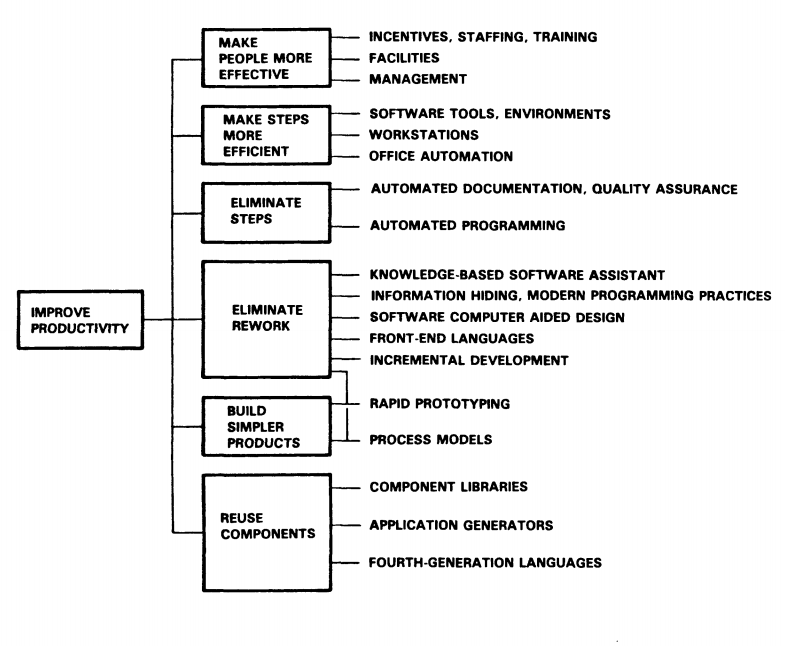
\includegraphics{ImprovingProductivity.PNG}

\section{Comparison to Traditional Waterfall Method}
suggest your ideas. 
-integration
-how we can produce more productivity
-customer involvement 
 
Comparison to traditional waterfall method and cost/productivity



Understanding and Controlling Software Costs:
-avoiding rework
-integrated support project environments 
-rapid prototyping through integration

paper QA in agile:
-QA suggests early and often, maybe more important at the start 
-Continuous integration prevents this, build quality debt
-Customer and development factors control software quality
-presented to customer early and often
-cycle time is almost constant to ensure software quality is always good


Software development life cycle AGILE vs traditional approaches
-again early customer involvement 
-delivers results quickly and more cost effectively 
-has diagrams comparison on costs and productivity 
-high customer involvement 




\section{Conclusion}

What we have concluded from this this work is that constant integration to avoid bugs with other methods for quality assurance [1][2] is definitely key too  high productivity

Write your conclusion here. The conclusion should do more than summarise the essay, making clear the contribution of the work and highlighting key points, limitations, and outstanding questions. It should not introduce any new content or information.

\bibliographystyle{ieeetran}
\bibliography{references}
[1] B. W. Boehm and P. N. Papaccio, "Understanding and controlling software costs," in IEEE Transactions on Software Engineering, vol. 14, no. 10, pp. 1462-1477, Oct 1988.
[2] S. Bhasin, "Quality Assurance in Agile: A Study towards Achieving Excellence," 2012 Agile India, Bengaluru, 2012, pp. 64-67.
doi: 10.1109/AgileIndia.2012.18
[3] R. Malhotra and A. Chug, "Comparative analysis of agile methods and iterative enhancement model in assessment of software maintenance," 2016 3rd International Conference on Computing for Sustainable Global Development (INDIACom), New Delhi, 2016, pp. 1271-1276.
[4] Ming Huo, J. Verner, Liming Zhu and M. A. Babar, "Software quality and agile methods," Proceedings of the 28th Annual International Computer Software and Applications Conference, 2004. COMPSAC 2004., 2004, pp. 520-525 vol.1.
[5] Clark, B., 1999. Effects of process maturity on development effort. unpublished paper available at http://sunset. usc. edu/~ bkclark/Research.
[6] Fowler, M. and Highsmith, J., 2001. The agile manifesto. Software Development, 9(8), pp.28-35.


\end{document}
